\documentclass{llncs}
\pagestyle{plain}
\usepackage[english]{babel}
\usepackage[utf8x]{inputenc}
\usepackage{amsmath}
\usepackage{graphicx}
\usepackage{url}
\usepackage[colorinlistoftodos]{todonotes}

\makeatletter
\newcommand*{\bdiv}{%
  \nonscript\mskip-\medmuskip\mkern5mu%
  \mathbin{\operator@font div}\penalty900\mkern5mu%
  \nonscript\mskip-\medmuskip
}
\makeatother

\title{Capturing the Ineffable:\\Collecting, Analysing and Automating Web Document Quality Assessments}
\author{Davide Ceolin\inst{1} and Lora Aroyo\inst{1} and Julia Noordegraaf\inst{2}}
\institute{\email{\{d.ceolin,lora.aroyo\}@vu.nl}\\VU University Amsterdam\\ de Boelelaan 1081a\\ 1081HV\\ Amsterdam, The Netherlands \and \email{j.j.noordegraaf@uva.nl} \\ University of Amsterdam}

\begin{document}
\maketitle
\begin{abstract}
Automatic estimation of the quality of Web documents is a challenging task, especially because the definition of quality heavily depends on the individuals who define it, on the context where it applies, and on the tasks at hand. 
In this paper, we investigate the quality of Web documents from two perspectives. Firstly, we propose a method for capturing Web quality assessments based on a nichesourcing Web application that we developed. Secondly, we investigate the characteristics of Web documents that hint at their quality levels. We propose a model for automatically estimating such assessments, we analyze users ability to judge quality based on features extracted from these documents and, finally, we decompose overall quality assessments so to identify which quality dimensions (e.g., accuracy, precision) are of higher importance when assessing Web documents.
We evaluate our contributions on two use cases involving experts (journalists and media scholars) that make professional use of Web documents. Our results show that: (1) it is possible to automate the process of Web document quality estimation to a level of high accuracy; (2) that document features shown in isolation are poorly informative to users; and (3) that, related to the tasks we propose (i.e., choosing Web documents to use as a source for writing an article on the vaccination debate), the most important quality dimensions are accuracy, trustworthiness, and precision.
\end{abstract}

\section{Introduction}
Automatically estimating the quality of Web documents is a compelling, yet intricate issue. It is compelling because the huge amount of Web documents we can access makes their manual evaluation a costly operation. So, to guarantee we access the best documents available on the Web on a given matter (or, at least, that the documents we observe meet some minimum qualitative standards), an automated assessment is needed.
However, quality is a rather inflated term, that assumes different meanings in different contexts and with different subjects. This is the reason why we call them ``ineffable''.

This paper aims at investigating how it is possible to capture such ineffable judgments and at understanding how they are characterized. In particular, our current focus is on the quality assessment of Web documents to be used for professional use (i.e., by journalists and media scholars). 
In the first part of the paper, we describe a nichesourcing application for collecting Web document quality assessments (WebQ\footnote{The tool is running at \url{http://webq3.herokuapp.com}, the code is available at~\url{https://github.com/davideceolin/webq}.}) that we developed. Then, we describe a thorough set of analyses we performed on the quality assessments gathered through WebQ by means of two user studies. From these analyses, we derive that quality assessments heavily depend on the task at hand. The subjectivity of such assessments is overcome by the fact that users share a common background and assess documents with the same task in mind. Hence, besides the individual peculiarities in the assessments, we can aggregate user contributions and actually automate their learning. This opens up for the possibility of extending the set of assessments to be used for training in the future.

The rest of the paper is structured as follows. Section~\ref{sec:related} introduces related work. Section~\ref{sec:webq} describes the nichesourcing Web application we developed for collecting quality assessments, WebQ.
Section~\ref{sec:results} describes the two case studies we performed, along with the results collected. These results are discussed in Section~\ref{sec:discussion}. Section~\ref{sec:conclusion} concludes the paper.


\section{Related Work}
\label{sec:related}

The problem of assessing the quality of Web documents and, more in general, (Web) data and information, is a compelling one and has been tackled in diverse contexts. 

The ISO 25010 Model~\cite{iso} is a standard model for data quality. From this model, we select those data quality dimensions from this model that apply also to Web documents (e.g., precision, accuracy) and ask the users of WebQ to rate Web documents on them. This set of quality dimensions has been extended to include other measures tailored to Web documents, like neutrality and readability.

The problem of identifying the documents of higher quality for a given purpose is common in information retrieval. Bharat et al~\cite{bharat2016method} copyrighted a method for clustering online news content based on freshness and quality of content. Clearly, their approach differs from ours as they focus on news, and they aim at clustering documents. However, one of the key features for determining the quality of documents is the (estimated) authoritativeness of the source, both in their and in our approach. Kang and Kim~\cite{Kang:2003:QTC:860435.860449}, instead, find links between specific quality requirements and user queries. We do not make use of queries since we preselect documents and also predefine the task the users are asked to perform. However, we still analyze user assessments to derive their specific definition of quality, and might consider analyzing user queries in the future, when we will expand the dataset and tasks at hand.

Following up on the use of specific metadata as markers for quality, Amento et al.~\cite{Amento:2000:LMQ:345508.345603} use link-based metrics to make quality predictions, showing that these perform as good as content-based ones. In our case, we focus mainly on metadata- and context-based features, and will consider link-based ones in the future.

Regarding the use of niche- or crowdsourcing for collecting information and, in particular, quality assessments, Lee et al.~\cite{Lee:2002:AMI:637474.637478} provide a framework tailored to organizations. Zhu et al.~\cite{zhu} propose a method for collaboratively assessing the quality of Web documents that shows some similarity with ours (e.g., we both collect collaborative quality assessments), but the assessments we aim at collecting are based on specific tasks, while they rely on contributions via browsers plugins. Currently, we focus on niches for collecting quality assessments. In the future, we will make use of crowdsourcing as well, embracing methods for extracting ground truth like the CrowdTruth framework~\cite{Inel2014}.


While this paper proposes a framework that aims at generically identifying markers for quality of Web documents, we evaluate such framework with an emphasis on digital humanities applications. Digital Humanities scholars are professionals that are used to critically evaluate the sources they deal with, hence we target this specific class of users to investigate how to extend source criticism practices to cover Web documents as well.
Source criticism is the process of evaluating traditional information sources that is common in the (digital) humanities. De Jong and Schellers~\cite{dejong} provide an overview of source criticism methods, evaluated in terms of predictive and congruent validity. We will advance such evaluations to identify which document features determine their quality.
This paper extends the work we presented at the Web Science conference, where we began the exploration of how it is possible to assess the quality of Web documents, especially for the Digital Humanities~\cite{Ceolin:2016:TWD:2908131.2908198}.

Lastly, one aspect that we partially consider when estimating the quality of Web document is their provenance. Provenance analysis is used to assess the quality of humanities sources, as Howell and Prevenier mention~\cite{provenance}. In Computer Science,
the use of provenance information to assess the quality of Web data has been explored by Hartig and Zhao~\cite{hartig}, who focus mostly on temporal qualities. More extensively, Zaveri et al.~\cite{LDQ} provide a review on quality assessment for Linked Data. We also investigated the assessment of crowdsourced annotations using provenance analysis~\cite{jdiq2015,ifiptm2015}. 

\section{Nichesourcing Web Document Quality Assessments}
\label{sec:webq}
We developed WebQ, a tool for investigating and collecting judgments about Web documents. WebQ aims at shedding a light on three main aspects:
\begin{itemize}
\item Understanding whether (professional) users are able to estimate the quality of Web documents based on limited sets of features of these documents (e.g., the sentiment of these documents, or the list of entities extracted from them);
\item Understanding whether user judgments are coherent enough over multiple documents and among diverse assessors, so to allow their automated learning;
\item Understanding how can overall quality assessments about Web documents be explained in terms of specific quality dimensions (i.e., understanding what is the weight of precision, accuracy, etc. when users provide overarching quality assessments about Web documents), when focusing on specific tasks.
\end{itemize}

\subsection{Document Features and Document Quality Dimensions}
We carachterize documents by means of features we automatically extract about them. In Section~\ref{sec:results} we analyze the existence of correlations between these automatically extracted features and the nichesourced qualities.
\subsubsection{Document Features} These are a series of attributes we automatically extract by means of Web APIs. These features aim at identifying commonalities among documents, opening up for the possibility of predicting their qualities (provided that features and qualities correlate). These features are:
\begin{description}
\item[Entities, Sentiment, Emotions] We use AlchemyAPI to extract all the features mentioned in the documents, along with their relevance to the document. Also, AlchemyAPI provides us with a quantification of the sentiment expressed by the document (positive or negative, and its strength), and its emotions (joy, fear, sadness, disgust and anger, along with their strength).
\item[Trustworthiness] This is an anomalous feature, because trustworthiness belongs also to the document qualities. In this case, we use the Web Of Trust API to obtain crowdsourced trustworthiness assessments about the source publishing the article.
\end{description}
\subsubsection{Document Quality Dimensions} These are a series of abstractions of these documents qualifying the information therein contained, namely:
\begin{description}
\item[Overall Quality] This score represents the overall reliability of the document.
\item[Accuracy] quantifies the level of truthfulness of the document information.
\item[Precision] quantifies whether the document information is precise.
\item[Completeness] determines whether the information contained in the document (or facts) are complete.
\item[Neutrality] determines whether a particular stance (e.g., pro or con a given topic) is represented in the document.
\item[Readability] quantifies whether the document reads well.
\item[Trustworthiness] quantifies the perceived level of trustworthiness of the information in the document. Note that the Web Of Trust score refers to the source, while this quality refers to the specific document evaluated.
\end{description}


\subsection{Structure of WebQ}

Below we describe the structure of WebQ, illustrated in Figure~\ref{fig:overview}.
\paragraph{Architecture}
The application is developed based on the Flask Python library~\footnote{\url{http://flask.pocoo.org/}}.
As backend storage for Web document assessments, we use MongoDB~\footnote{\url{http://mongodb.com}}.
\paragraph{Annotations}
We use AnnotatorJs\footnote{\url{http://annotatorjs.org}} as a tool for allowing our users to indicate which specific parts of a document mark particular qualities of the whole document.
AnnotatorJs is a javascript library ran on the client side. This library records the document annotations by sending HTTP messages to a storage server. We adapted to this purpose the Annotation Store\footnote{\url{https://github.com/openannotation/annotator-store}}, which relies on ElasticSearch for storage and retrieval of annotations.
\paragraph{HTTP Proxy}
We developed an HTTP proxy to provide to the users with the Web documents to be annotated within WebQ. This proxy allows to present the documents within our application and allowing users to annotate them by enabling AnnotatorJs. In this manner, the users see the exact same document they would see on the Web, but they are able to annotate it, remaining in the context of our application.
This proxy is tailored to the documents we identified in our dataset and is able to render them at their best. In particular, it addresses the following issues:
\begin{itemize}
\item replace relative paths with absolute ones in image, CSS and link addresses (so that the page can refer to the absolute addresses of the accessory files);
\item handle charsets: to properly render the documents, their charset has to be correctly detected and utilized;
\item forward the browser headers. Some websites allow being accessed only via (some) browsers, and not being scraped. Our proxy accesses them programmatically, but on behalf of a browser access. Therefore, we forward the browser headers to the URL via the proxy;
\end{itemize}
In the future, we aim at extending our dataset, so we will work on further extensions of this proxy.
\paragraph{Randomizer}
WebQ is designed for collecting Web document quality assessments via one or more user studies. In such a scenario, users would access the application more or less simultaneously. We assign to each user a random sequence of documents to assess (we set the length of such sequence to six), but at the same time we also need to guarantee that the dataset is uniformly assessed: documents should get approximatively $$ n_{assessments} = |dataset |  \bdiv | {\it users} | $$ assessments, where $| dataset|$ is the cardinality of the document dataset (50), $\bdiv$ is the integer division and $| {users}|$ is the cardinality of the set of users. 

Before running the user studies, we generate $n_{assessments}$ random permutations of documents. We split such sequences in consecutive sequences of 6 documents. Sequences are then uniquely assigned to users as soon as they register in the application.

\begin{figure}
\centering
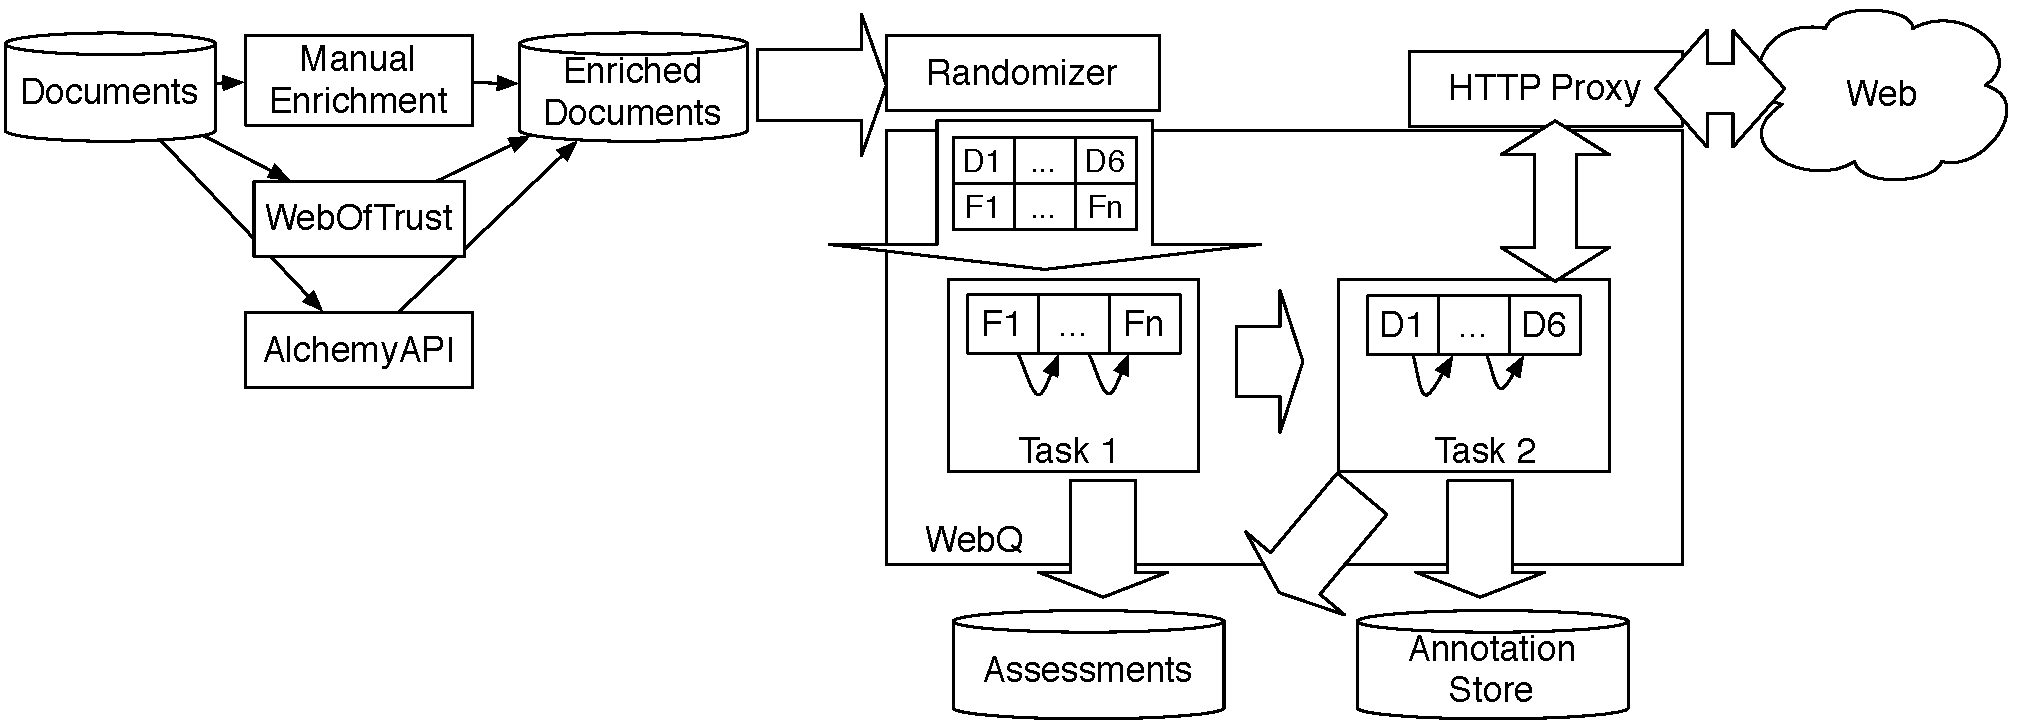
\includegraphics[width=0.70\textwidth]{overview.pdf}
\caption{Overview of the WebQ application. The document set is firstly enriched by using AlchemyApi, Web of Trust and manual enrichment. Then, a random selection of six documents is presented to the users for the first task: selecting the documents with the highest quality on the basis of the value of one document feature. After all the features (sentiment, entities, etc.) have been evaluated, then users are asked to assess each of the six documents assigned (task 2). In this case, documents are rendered through an HTTP proxy, to allow annotating them and visualizing the documents within the app.\label{fig:overview}}
\end{figure}

\subsection{Tasks Description}
In WebQ we ask the users to perform two tasks. The first task aims at exploring whether document features could be used as quality indicators alone. The second task aims at collecting assessments about the documents presented. The two tasks are described as follows.


\paragraph{Task 1}
The application is divided into two tasks. In the first, task we evaluate the informativeness of specific document features in relation to the quality of the documents.
The task is structured as follows:
\begin{enumerate}
\item We assign to each user a set of six documents from our overall dataset.
\item We identify six classes of potentially useful features about the documents, namely: the document's sentiment and emotions expressed, its trustworthiness, its title, its source and the list of entities we extract from it.
\item In turn, we show the values for each of these features to the user, i.e., first we present the user with the six lists of entities extracted from the six documents (one list per document), then we present the user with the sentiment and the emotions detected in each document, and so on. Each time only one feature is presented. Note that the selection of documents is fixed per user. However, the user does not know the documents, they only know the values of the features we present. Also, every time we present features to the users we shuffle the document order and we use different identifiers.
\item We ask the user to select which documents among these six she will use as a source for her article, based on the information displayed.
\item Lastly, we ask the user to make the same selection on the basis of all the features presented together.
\end{enumerate}

\paragraph{Task 2}
We ask the user to assess the quality of each article in depth. Based on the same selection of six articles the user was assigned to in task 1, they:
\begin{enumerate}
\item Read the article
\item Assess the overall quality of the article, as well as the following quality dimensions: accuracy, precision, completeness, readability, neutrality, trustworthiness. Assessments are indicated in a 1 to 5 Likert scale.
\item Highlight in the article the words or sentences that motivate their assessments, tagging each selection with the name of the corresponding quality dimension and with an indication of the fact that the selection represents a positive or negative observation.
\item Revise their quality assessments (step 2.) if they wish so.
\end{enumerate}

\section{Case Studies}
\label{sec:results}
In this section, we describe the two case studies we run. Both case studies are based on the same set of documents, which we describe as follows.
\subsection{Dataset and Scenario}
The dataset we base our experiments on is composed by Web documents about the vaccination debate that has been triggered by the measles outbreak happened at Disneyland, California, in 2015\footnote{The dataset is available at~\url{https://goo.gl/cLDTtS}}. This dataset contains 50 documents, which are diversified in terms of:
\begin{description}
\item[Stance] Some are pro vaccinations, some con, some neutral.
\item[Type of source] We include in our dataset diverse types of sources, comprising official reports from authorities, news articles, editorial articles, blog posts.
\end{description}

The scenario we hypothesize is that users have to write an article about the vaccination debate triggered by such measles outbreak. We propose diverse types of Web documents to the users, and we ask to select those they would use as a source for their article (i.e., those they consider of a higher quality).

\subsection{Case Study 1 - Journalism Students}
\subsubsection{Experimental Setup} The first case study involved a class of 20 last-year journalism students from the University of Amsterdam. The students performed both tasks of WebQ in a time frame that lasted between 45 and 60 minutes.
\subsubsection{Results} We present here a series of analyses on the results collected. 
\paragraph{Document Assessments Collected} In this first experiment we collected 104 complete assessments (i.e., quality judgments about the diverse quality dimensions of the documents) and 238 annotations.
\paragraph{Comparison of the two document assessments in task 2}
In task 2 we ask the users to assess the documents two times: the first time they read the documents, and after having highlighted the motivations for their assessments. We observe no significant difference between these two assessments, using a Wilcoxon Signed-rank test at 95\% confidence level.
\paragraph{Document Assessments Predictability}
The first analysis we perform regards the predictability of Web documents assessments. Only two or three assessments are provided per document, but if users assess the documents coherently enough (i.e., following similar policies), and if the features we extracted (entities, sentiment, emotions, trustworthiness) are considered by the users' policies, then we might be able to automatically learn such predictions.
Table~\ref{tab:predj} shows the results of such predictions using the Support Vector Classification algorithm.
\begin{table}
\centering
\caption{Results of 10-fold cross-validation using Support Vector Classification with different number of features, and predicting either 5 classes (as in the 1-5 Likert scale used in WebQ) or 2 classes (i.e., high- and low-quality documents). We calculated the performance for all possible permutations of the four classes of features. For each cardinality of such permutation (1,2,3,4) we show the best performing combination.\label{tab:predj}}
\begin{tabular}{|l|c|c|}
\hline
{\bf Features used} & {\bf SVC 5 classes} & {\bf SVC 2 classes}\\
\hline
trustworthiness & 48\% & 75\%\\
\hline
sentiment, trustworthiness & 46\% & 78\%\\
\hline
sentiment, emotions, trustworthiness & 38\% & 72\%\\
\hline
sentiment, emotions, trustworthiness, entities & 39\% & 72\%\\
\hline
\end{tabular}
\end{table}

\paragraph{Correlation between quality dimensions and overall quality}

We checked the correlation between the overall quality score and the scores given to each quality dimensions. Results are reported in Table~\ref{tab:corrj}.
\begin{table}
\centering
\caption{Correlation between each quality dimension and the overall quality score attributed to the documents.\label{tab:corrj}}
\begin{tabular}{|l|c|}
\hline
{\bf Quality dimension} & {\bf Correlation with Overall Quality} \\
\hline
Accuracy         &      0.89\\ \hline
Completeness     &      0.69\\ \hline  
Neutrality       &      0.46\\ \hline  
Relevance        &      0.63\\ \hline  
Trustworthiness  &      0.80\\ \hline  
Readability      &      0.67\\ \hline 
Precision        &      0.77\\ \hline 
\end{tabular}

\end{table}

\paragraph{Correlation between document selection (task 1) and document assessments (task2)}
In task 1 we ask the users to select documents they think are of high quality based on diverse features we extracted from these documents. If many users select a document, we might derive that it has high probability to be of high quality. Since each document has been proposed to only either two or three users, we compute such probability using a smoothing factor that allows to account for the uncertainty due to the small samples observed (see Equation~\eqref{eq:smoothing}). Also, smoothing allows us to treat differently documents that have been proposed two or three times: if a document has never been selected when it has been proposed two times, its probability to be of high quality is 0.25; if it has been proposed three times, 0.2. This probability is equivalent to the expected value of a Beta probability distribution with a non-informative prior (as we do not know a priori which documents are of higher quality).
\begin{equation}
P = \frac{\# selection +1}{\# samples + 2}
\label{eq:smoothing}
\end{equation}

In task 2, users assess these same documents. Table~\ref{tab:t1t2corrj} reports the correlation between the probability from task 1 and the overall quality score from task 2.

\begin{table}
\centering
\caption{Correlation between the probability of documents to be selected in task 1 and their overall quality assessment from task 2.\label{tab:t1t2corrj}}
\begin{tabular}{|l|c|}
\hline
{\bf Feature shown } & {\bf Correlation (Spearman)}  \\
{\bf to the users (task 1)} & {\bf with Overall Quality (task 2)}\\
\hline
Entities & -0.07 \\ \hline
Sentiment & 0.09 \\ \hline
Trustworthiness & 0.20 \\ \hline
Sources & 0.29 \\ \hline
Title & -0.07 \\ \hline
All & 0.20 \\ \hline
\end{tabular}
\end{table}

\paragraph{User Evaluation}
We asked the users express their opinion about the experiment by means of a questionnaire. The quantitative results of the 13 respondent (52\% of the total) are reported in Table~\ref{tab:questj}. To those results, we can add that trustworthiness, accuracy and the source of the document are the features mostly indicated by the users as good quality markers.

\begin{table}
\centering
\caption{Results of the user evaluation questionnaire.\label{tab:questj}}
\begin{tabular}{|p{6.2cm}|c|c|c|c|c|}
\hline
{\bf Question} & \multicolumn{5}{c|}{\bf Result} \\ \cline{2-6}
& {\bf 1 (bad)} & {\bf 2} & {\bf 3} & {\bf 4} & {\bf 5 (good)} \\ \hline
How was your experience? & {\bf 30.8\%} & {\bf 30.8\%} & 23.1\% & 15.4\% & 0\%\\ \hline
Was the experience easy? & 15.4\% & {\bf 53.8}\% & 23.1\% & 7.7\% & 0\% \\ \hline
Does this experiment resemble the process that you would follow when you write an article? & {\bf 38.5\%} & 30.8\% & 23.1\% & 7.7\% & 0\% \\ \hline
Do you think that the entities extracted from the Web documents are good quality markers? & 15.4\% & 15.4\% & {\bf 30.8\%} & {\bf 30.8\%} &  0\% \\ \hline
\end{tabular}
\end{table}

\paragraph{Quality Definition and Qualitative Analysis of Annotations and Remarks}
Lastly, from a qualitative evaluation of the annotations and of the remarks collected, we can derive that users assume that \emph{the documents of higher quality are those showing the following qualities: high trustworthiness, high accuracy and high precision}.

\subsection{Case Study 2 - Media Scholars}
\subsubsection{Experimental Setup}
The second case study involves 20 media scholars attending the Research School for Media Studies (RMeS) summer school.
We present the users with a setting that closely resembles the one adopted for case study 1 but, following the indications received from the user evaluation, we adopt the following improvements:
\begin{itemize}
\item we improve the user introduction and add a walk-through session to guide the users in the application;
\item task descriptions and user experience are improved (e.g., landing pages).
\end{itemize}
The users had about 45 minutes at their disposal to complete the two tasks.

\subsubsection{Results} We present the results obtained and their analyses following the same structure adopted for case study 1.
\paragraph{Document Assessments Collected} In this experiment we collected 47 complete assessments about the documents in our dataset and 89 annotations.
\paragraph{Comparison of the two document assessments in task 2} Also in this case we observe no significance difference between the first and the second series of assessments, for any quality dimension.
\paragraph{Document Assessments Predictability} Like with the previous case study, we use 10-fold cross-validation to test the predictability performance of Support Vector Classifier on the overall quality assessment. 
Results are reported in Table~\ref{tab:predm}.
\begin{table}
\centering
\caption{Accuracy of the prediction of the overall quality assessments on the second case study. We compute all features permutations and we show the best performing combination per feature set cardinality (1,2,3,4).\label{tab:predm}}
\begin{tabular}{|l|c|c|}
\hline
{\bf Features used} & {\bf SVC 5 classes} & {\bf SVC 2 classes} \\ \hline
trustworthiness & 63\% & 89\% \\ \hline
sentiment, trustworthiness & 53\% & 86\% \\ \hline
sentiment, entities, trustworthiness & 34\% & 85\% \\ \hline
sentiment, entities, trustworthiness, emotions & 34\% & 85\% \\ \hline
\end{tabular}
\end{table}

\paragraph{Correlation between quality dimensions and overall quality}

We checked the correlation between the overall quality score and the scores given to each quality dimensions. Results are reported in Table~\ref{tab:corrm}.
\begin{table}
\centering
\caption{Correlation between each quality dimension and the overall quality score attributed to the documents.\label{tab:corrm}}
\begin{tabular}{|l|c|}
\hline
{\bf Quality dimension} & {\bf Correlation with Overall Quality} \\
\hline
Accuracy         &      0.89\\ \hline
Completeness     &      0.69\\ \hline  
Neutrality       &      0.45\\ \hline  
Relevance        &      0.64\\ \hline  
Trustworthiness  &      0.78\\ \hline  
Readability      &      0.66\\ \hline 
Precision        &      0.76\\ \hline 
\end{tabular}

\end{table}

\paragraph{Correlation between document selection (task 1) and document assessments (task2)}
We computed the probability of documents to be of high quality based on the number of selections they received in task 1, as indicated by Equation~\eqref{eq:smoothing}.
Table~\ref{tab:t1t2corrm} reports the correlation between such probability and the overall quality score from task 2.

\begin{table}
\centering
\caption{Correlation between the probability of documents to be selected in task 1 and their overall quality assessment from task 2.\label{tab:t1t2corrm}}
\begin{tabular}{|l|c|}
\hline
{\bf Feature shown } & {\bf Correlation (Spearman)}  \\
{\bf to the users (task 1)} & {\bf with Overall Quality (task 2)}\\
\hline
Entities & 0.38 \\ \hline
Sentiment & 0.19 \\ \hline
Trustworthiness & 0.21 \\ \hline
Sources & 0.25 \\ \hline
Title & 0.15 \\ \hline
All & 0.24 \\ \hline
\end{tabular}
\end{table}

\paragraph{User Evaluation}
The results of the user evaluation questionnaire are reported in Table~\ref{tab:questm}. To these quantitative results, we add the fact that users indicate accuracy and also indicators from social media (e.g., discussion on the topic, likes) as possible quality markers. The results described here are based on a very little sample, since only four participants responded to the questionnaire.
\begin{table}
\centering
\caption{Results of the user evaluation questionnaire.\label{tab:questm}}
\begin{tabular}{|p{6.2cm}|c|c|c|c|c|}
\hline
{\bf Question} & \multicolumn{5}{c|}{\bf Result} \\ \cline{2-6}
& {\bf 1 (bad)} & {\bf 2} & {\bf 3} & {\bf 4} & {\bf 5 (good)} \\ \hline
How was your experience? & {\bf 25\%} & 0\% & {\bf 75\%} & 0\% & 0\%\\ \hline
Was the experience easy? & 0\% & {\bf 50}\% & {\bf 50\%} & 0\% & 0\% \\ \hline
Does this experiment resemble the process that you would follow when you write an article? & {\bf 50\%} & 0\% & 25\% & 25\% & 0\% \\ \hline
Do you think that the entities extracted from the Web documents are good quality markers? & {\bf 50\%} & 25\% & 0\% & 25\% &  0\% \\ \hline
\end{tabular}


\end{table}

\paragraph{Quality Definition and Qualitative Analysis of Annotations and Remarks}
Lastly, from a qualitative evaluation of the annotations and of the remarks collected, we can derive that users assume that \emph{the documents of higher quality are those showing the following qualities: high trustworthiness (e.g., expressed by the author's authoritativeness), high accuracy and high precision}.

\subsection{Comparison between Case Study 1 and 2}
We compare the results obtained in case study 1 and 2.
First of all, we use a Wilcoxon signed-rank test to compare the performance obtained by support vector machines (Tables~\ref{tab:predj} and~\ref{tab:predm}). We observe no significant difference neither with 2 nor with 5 classes.

Also comparing the correlations between the quality dimensions and the overall quality (Tables~\ref{tab:corrj} and~\ref{tab:corrm}), we observe no significant difference.

Neither the results of Tables~\ref{tab:t1t2corrj} and~\ref{tab:t1t2corrm}, i.e., the correlation between probabilities of a document to be selected and its quality show any significant difference between task 1 and 2.

The second user questionnaire has been fulfilled only by a very limited number of users. A Wilcoxon signed rank test and a $\chi^2$ test both agree that the results from the two case studies are not significantly different, but the sample sizes are so small that we can hardly rely on these results.
\section{Discussion}
\label{sec:discussion}
We discuss here the results presented in Section~\ref{sec:results}.
We summarize the discussion by means of a series of statements that emerge from the analysis of the result. Each statement is presented and motivated below.
\paragraph{{\bf User assessments are stable and coherent.}} In both case studies, we observe that the first and the second document assessments are not significantly different. Moreover, in both cases, we can use Support Vector Classifier to automatically learn and predict the quality of documents. This means that, even if users assess different documents (the same document has been assessed by three users at most), assessments are coherent enough to be learned. Also, the features we identified (entities, sentiment, emotions, trustworthiness) correlate with these judgments enough to allow using them as features for prediction. 
\paragraph{{\bf User assessments are highly related to the task at hand.}}
The extremely high similarity between the results in Tables~\ref{tab:corrj} and~\ref{tab:t1t2corrm} shows that, when assessing the quality of documents, the task at hand is the most important factor. In fact, here the users were asked to pretend they were writing an article about the vaccination debate. Consequently, they focused on identifying the most accurate and trustworthy documents. Neutrality is the least significant quality of these documents because, if users want to represent the whole spectrum of the debate, they have to consider also the least neutral documents, provided that they are accurate enough. Different tasks could (and would probably) imply different quality requirements.

This opens up for the possibility to extend our training set with assessments from future experiments. In fact, the fact that the task is the most important aspect in such assessments makes new assessments datasets from future experiments assimilable to the existing one. In this manner, we will be able to scale up our current approach at Web scale.
In this light, although in some cases we observe that by considering only a subset of features we obtain a better performance (up to +6\% in some cases), we still prefer to consider all the features we collected so far. In fact, we do not know if, by extending the set of documents considered (or by diversifying the tasks at hand), some of the features that are now less significant could become more prominent.

\paragraph{{\bf Features in isolation are hardly meaningful (but the user experience plays a role here).}}
Entities, sentiment, and emotions, trustworthiness, title and source are hardly useful to be used to decide if a document is of high quality or not. The fact that these features are profitably used to learn the quality assessments of the documents using SVC means that they are good markers of quality (e.g., the fact that a given document expresses an extremely positive sentiment or show specific entities is correlated with its quality). Nevertheless, users are hardly able to determine the document quality on the basis of a quantification of such features. True is that in the second case study, although the performance is still pretty low, the results are slightly better than those of the first use case. This might be due to the different user background, but we believe that also the changes we added to WebQ facilitated such improvement.

\paragraph{{\bf The application setup should take (also) the user experience into consideration}}
We aim at collecting annotations from users, so we need to balance a couple of trade-offs between the application (and, hence, our) requirements and user-based constraints. First of all, our target users have a professional background that is not necessarily an Information or Computer Science background. So, even if the application is able to capture all the necessary information, the way its functionality is presented and the user is guided plays an important role. In fact, we observed (both via the questionnaire and via a post-study discussion) an improvement in the experience perception from case study 1 to 2. Moreover, our goal is to collect as many assessments as possible, but we have to take into account also that user attention decrease over time. This is the reason why in the second case study users paid more attention to the tasks performed, so provided much fewer assessments than in case study 1.

\section{Conclusion}
\label{sec:conclusion}

Automatically assessing the quality of Web documents is a crucial task to be able to benefit from the vast amount of information we can access online. In this paper, we investigated how we can collect quality assessments by means of a nichesourcing application we developed. We design and evaluate the application by means of two case studies involving journalists and media scholars. Such application provides all the necessary functionalities to collect such assessments (e.g., the possibility to rate and annotate documents) and the evaluations collected allowed us fine tuning it. Also, by analyzing the assessments collected in detail, we discovered that having a clearly defined task at hand we can overcome the subjectivity in document assessment, thus allowing assessments to be automatically estimated. In the specific task performed (selecting documents to be used as a source for an article on the vaccination debate), the most important quality dimensions considered are accuracy, precision and trustworthiness. We also show that the results collected in the two case studies are assimilable and allow creating a uniform collection of document assessments.

We plan to extend our application in several directions. We aim at considering other typologies of professional users, and at extending the tasks evaluated. Clearly, we intend to extend also the dataset of documents considered, as well as we will incorporate additional features in our models, including link- and network-based features (e.g., based on document interlinking) and social media-based features (e.g., the number of likes a given article received on social media sites, or the number of followers a given blog has). Lastly, as a consequence of such extension of both the number of records and of features, we will have to consider methods for scale our prediction models.

\subsubsection{Acknowledgements} This work was supported by the Amsterdam Academic Alliance Data Science (AAA-DS) Program Award to the UvA and VU Universities.
We thank the students of the UvA journalism course and the RMeS summer school participants for participating our user studies. 

\bibliographystyle{abbrv}
\bibliography{biblio} 

\end{document}